\documentclass[subscriptcorrection,upint,varvw,barcolor=Goldenrod3,mathalfa=cal=euler,balance,hyphenate,french,pdf-a]{asmejour}

\def\versionno{0.1}

\hypersetup{
	pdfauthor={Sesha Charla},                       		   	% <=== change to YOUR name[s]!
	pdftitle={Modelling and Parameter Estimation of Diesel Engine After-treatment System under Catalyst Saturation
	for Aging Diagnostics},                  	% <=== change to YOUR pdf file title
	pdfkeywords={Diesel Engnine Aftertreatment Systems, Diagnostics, Modelling, Nonlinear systems, System Identification, },% <=== change to YOUR pdf keywords
	pdfsubject = {Mathematical Modelling, Identification and Diagnostics},			% <=== change to YOUR subject
}


\JourName{Dynamic Systems, Measurement, and Control }%<=== change to the name of your journal

\PaperYear{2025}

% Custom Stuff
\input{ltx_core/ltx_pkgs.tex}
\input{ltx_core/new_cmds.tex}

\begin{document}
%=======================================================================================================================
\SetAuthorBlock{Sesha Charla}{School of Mechanical Engineering,\\
   Purdue University,\\
   West Lafayette, Indiana, USA\\
   email: scharla@purdue.edu}

\SetAuthorBlock{Peter H. Meckl\CorrespondingAuthor}{%
Fellow ASME\\
School of Mechanical Engineering,\\
Purdue University,\\
West Lafayette, Indiana, USA\\
email: meckl@purdue.edu
}

\SetAuthorBlock{Bin Yao}{%
Fellow ASME\\
School of Mechanical Engineering,\\
Purdue University,\\
West Lafayette, Indiana, USA\\
email: byao@purdue.edu
}
%=======================================================================================================================
\title{Modelling and Parameter Estimation of Diesel Engine After-treatment System under Catalyst Saturation for Aging
Diagnostics}

\keywords{Diesel Engine Aftertreatment System, System Identification, Nonlinear Systems, Hybrid Systems, Diagnostics, Parameter Estimation, Linear Programming.}

%=======================================================================================================================
%% Abstract should be no more than 250 words
\begin{abstract}
This work develops a reduced-order nonlinear discrete model from first principles to describe the dynamics of a diesel
engine's SCR catalyst under ammonia saturation. A novel parameter estimation algorithm is proposed utilizing the
relationship between predicted and measured $NO_x$ reduction in the system while explicitly considering the
uncertainties due to $NO_x$ sensor cross-sensitivity. The model forms part of a discrete nonlinear switched framework
that captures catalyst reaction dynamics, switching between saturation and desaturation modes depending on urea dosing.
By explicitly accounting for the interplay between residence time and sampling, the model parameters provide insights
into quantifying catalyst's aging.

\end{abstract}

%=======================================================================================================================
\date{Version \versionno , \today}
\maketitle
%=======================================================================================================================

\section{Intorduction}

Diesel engine after-treatment systems diminish the emission of harmful gases such as $NO_x$ and $CO$ from exhaust gases.
The Selective Catalytic Reduction (SCR) system chemically converts $NO_x$ into $N_2$ and $H_2O$, utilizing ammonia as a
reducing agent in the presence of a catalyst. This catalytic conversion process is regulated to decrease the levels of
ammonia in the exhaust, known as Ammonia Slip. Additionally, a catalytic reaction the Ammonia Slip Catalysis(ASC) is
also used to oxidize any excess ammonia at the end of the SCR bed. Figure-\ref{fig:exhaust_scheme} shows a schematic of
the SCR-ASC system. It is found that $No_x$-reduction capacity of the catalyst reduces with time due to hydro-thermal
aging and deposition of contaminants such as excess urea, platinum, sulfur and phosphorous \cite{jain2023diagnostics}.
The catalyst aging is a critical issue in the SCR-ASC system, as it can lead to reduction in the efficacy of conversion
and increased ammonia slip. A fault detection system that can detect the aging of the catalyst would provide better
control over the maintenance of the system and improve the overall reduction in emissions.

\begin{figure}[ht]
    \centering
    \includegraphics[width=0.45\textwidth]{./figs/1_intro/SCR-ASC_ModelReduction.png}
    \caption{Schematic of the SCR-ASC system}
    \label{fig:exhaust_scheme}
\end{figure}

Thus, modern diesel after-treatment systems, particularly those that integrate Selective Catalytic Reduction (SCR) with
Ammonia Slip Catalyst (ASC), necessitate advanced on-board diagnostics (OBD) tools for accurate assessment of SCR
degradation levels. However, the effectiveness of traditional OBD approaches for this purpose has been impeded by the
absence of model validation with real-world catalyst degradation data and the limitations imposed by existing commercial
$NO_x$ sensors' cross-sensitivity to ammonia.

Numerous studies have been conducted on modeling the SCR-ASC systems and their control \cite{yuan2015diesel}. A
prevalent modeling approach is to approximate the PDE model from the plug flow reactor assumption into a set of ODEs
using the idealization of the plug-flow reactor into a sequence of Continuously Stirred Tank Reactors (CSTRs)
(\cite{hsieh2011development}, and \cite{nova2014urea}). This discretization requires at least 2 CSTRs to capture the
system dynamics and causality, thereby increasing the model order. The single CSTR approach was first justified in
\cite{devarakonda2008adequacy} and a nonlinear model was developed using these assumptions, which was then linearized
for feedback control design (\cite{devarakonda2009model}). With this model, observers were designed to estimate the
states corresponding to the catalyst's storage (\cite{ma2017observer}, \cite{jain2020term}). A method for detecting the
catalyst's aging by observing the change in the maximum storage capacity of the catalyst, modeled as an exponential
function of temperature, was also proposed in \cite{ma2017observer}. A common theme in these studies is the resulting
non-convex, nonlinear parameter estimation problem. Moreover, these studies assume the availability of all the gaseous
states at the tail-pipe to eliminate the effects of cross-sensitivity of the $NO_x$ sensors, which is not always the
case in real-world applications. One other fundamental issue with a single cell CSTR assumption is that it results in
the causality reversal at the reaction rates as CSTR inherently assumes that the output concentrations are the same as
CSTR's accumulator concentrations \cite{charla2024reduced}.

An alternative approach to the problem would be discarding the CSTR assumption and modelling the time evolution of the
sensor signals when a "plug" or "parcel" of the exhaust gases flows through the chamber in discrete time considering the
interplay between sampling and residence time of the reactants. The catalyst saturation that is inherently considered in
the CSTR approach needs to be explicitly included as separate mode of the system. The present work developed such a
model under catalyst saturation which becomes one of the modes of the complete switched nonlinear model. Following the
model development we present the parameter estimation algorithm that estimates the parameters of the saturated catalyst
model using the real-world data whose operating mode is unknown and has additional uncertainties due to $NO_x$ sensor's
cross-sensitivity to ammonia.

\section{SCR-ASC System Dynamics Under Catalyst Saturation}
%==
The SCR-ASC subsystem in the diesel engine after-treatment systems involves reacting flow on the top of a catalyst which
adsorbs ammonia from urea decomposition. The reaction kinetics start with the decomposition of urea into ammonia
followed by its adsorption onto the surface of the catalyst. The $NO_x$ entering the chamber is reduced by this adsorbed
ammonia. The Eley-Rideal reaction mechanism \cite{yuan2015diesel}, \cite{hsieh2011development}, \cite{nova2014urea} is
considered for modeling the SCR reaction kinetics, where one reactant $(NO_x)$ is gaseous, and the other is adsorbed on
the catalyst surface $(NH_3)$. \cite{nova2014urea} lists all the reactions that take place inside the
SCR-ASC chamber. Ammonia oxidation (AMOX) happens both on the surfaces of the SCR catalyst and the ASC catalyst in the
mechanism that is similar, but SCR catalyst favors $NO_x$ reduction while ASC is specifically designed for ammonia
oxidation.
In order to keep the model order reasonably low and parameters identifiable, only the following three prominent reactions \cite{devarakonda2008adequacy},\cite{hsieh2011development} are considered:
\begin{enumerate}
    \item Standard SCR reaction:
    \begin{align*}
        4 NH_3 ^{ads} + 4 NO + O_2 &\xrightarrow[]{k_{scr}} 4 N_2 + 6 H_2O %\label{eqn::std_scr}
        & \lrf{1}
    \end{align*}
    \item Ammonia Oxidation:
    \begin{align*}
        4 NH_3^{ads} + 3 O_2 &\xrightarrow[]{k_{oxi}} 2 N_2 + 6 H_2O %\label{eqn::amox}
        & \lrf{2}
    \end{align*}
    \item Ammonia Adsorption/Desorption:
        \begin{align*}
            NH_3 + \Theta_{free} &\xrightleftharpoons[k_{des}]{k_{ads}} NH_3^{ads}
            %\label{eqn::ads}
            & \lrf{3}
        \end{align*}
\end{enumerate}
%==
This aggregation of reactions results in errors in parameter estimates, specifically parameters containing rate constant
for the $NO_x$ reduction $\lr{k_{scr}}$ will have higher (bounded) uncertainty as it becomes dependent on the nitrogen
selectivity of AMOX reaction \cite{jain2023diagnostics}.
%=======================================================================================================================
\begin{figure}[ht]
    \centering
    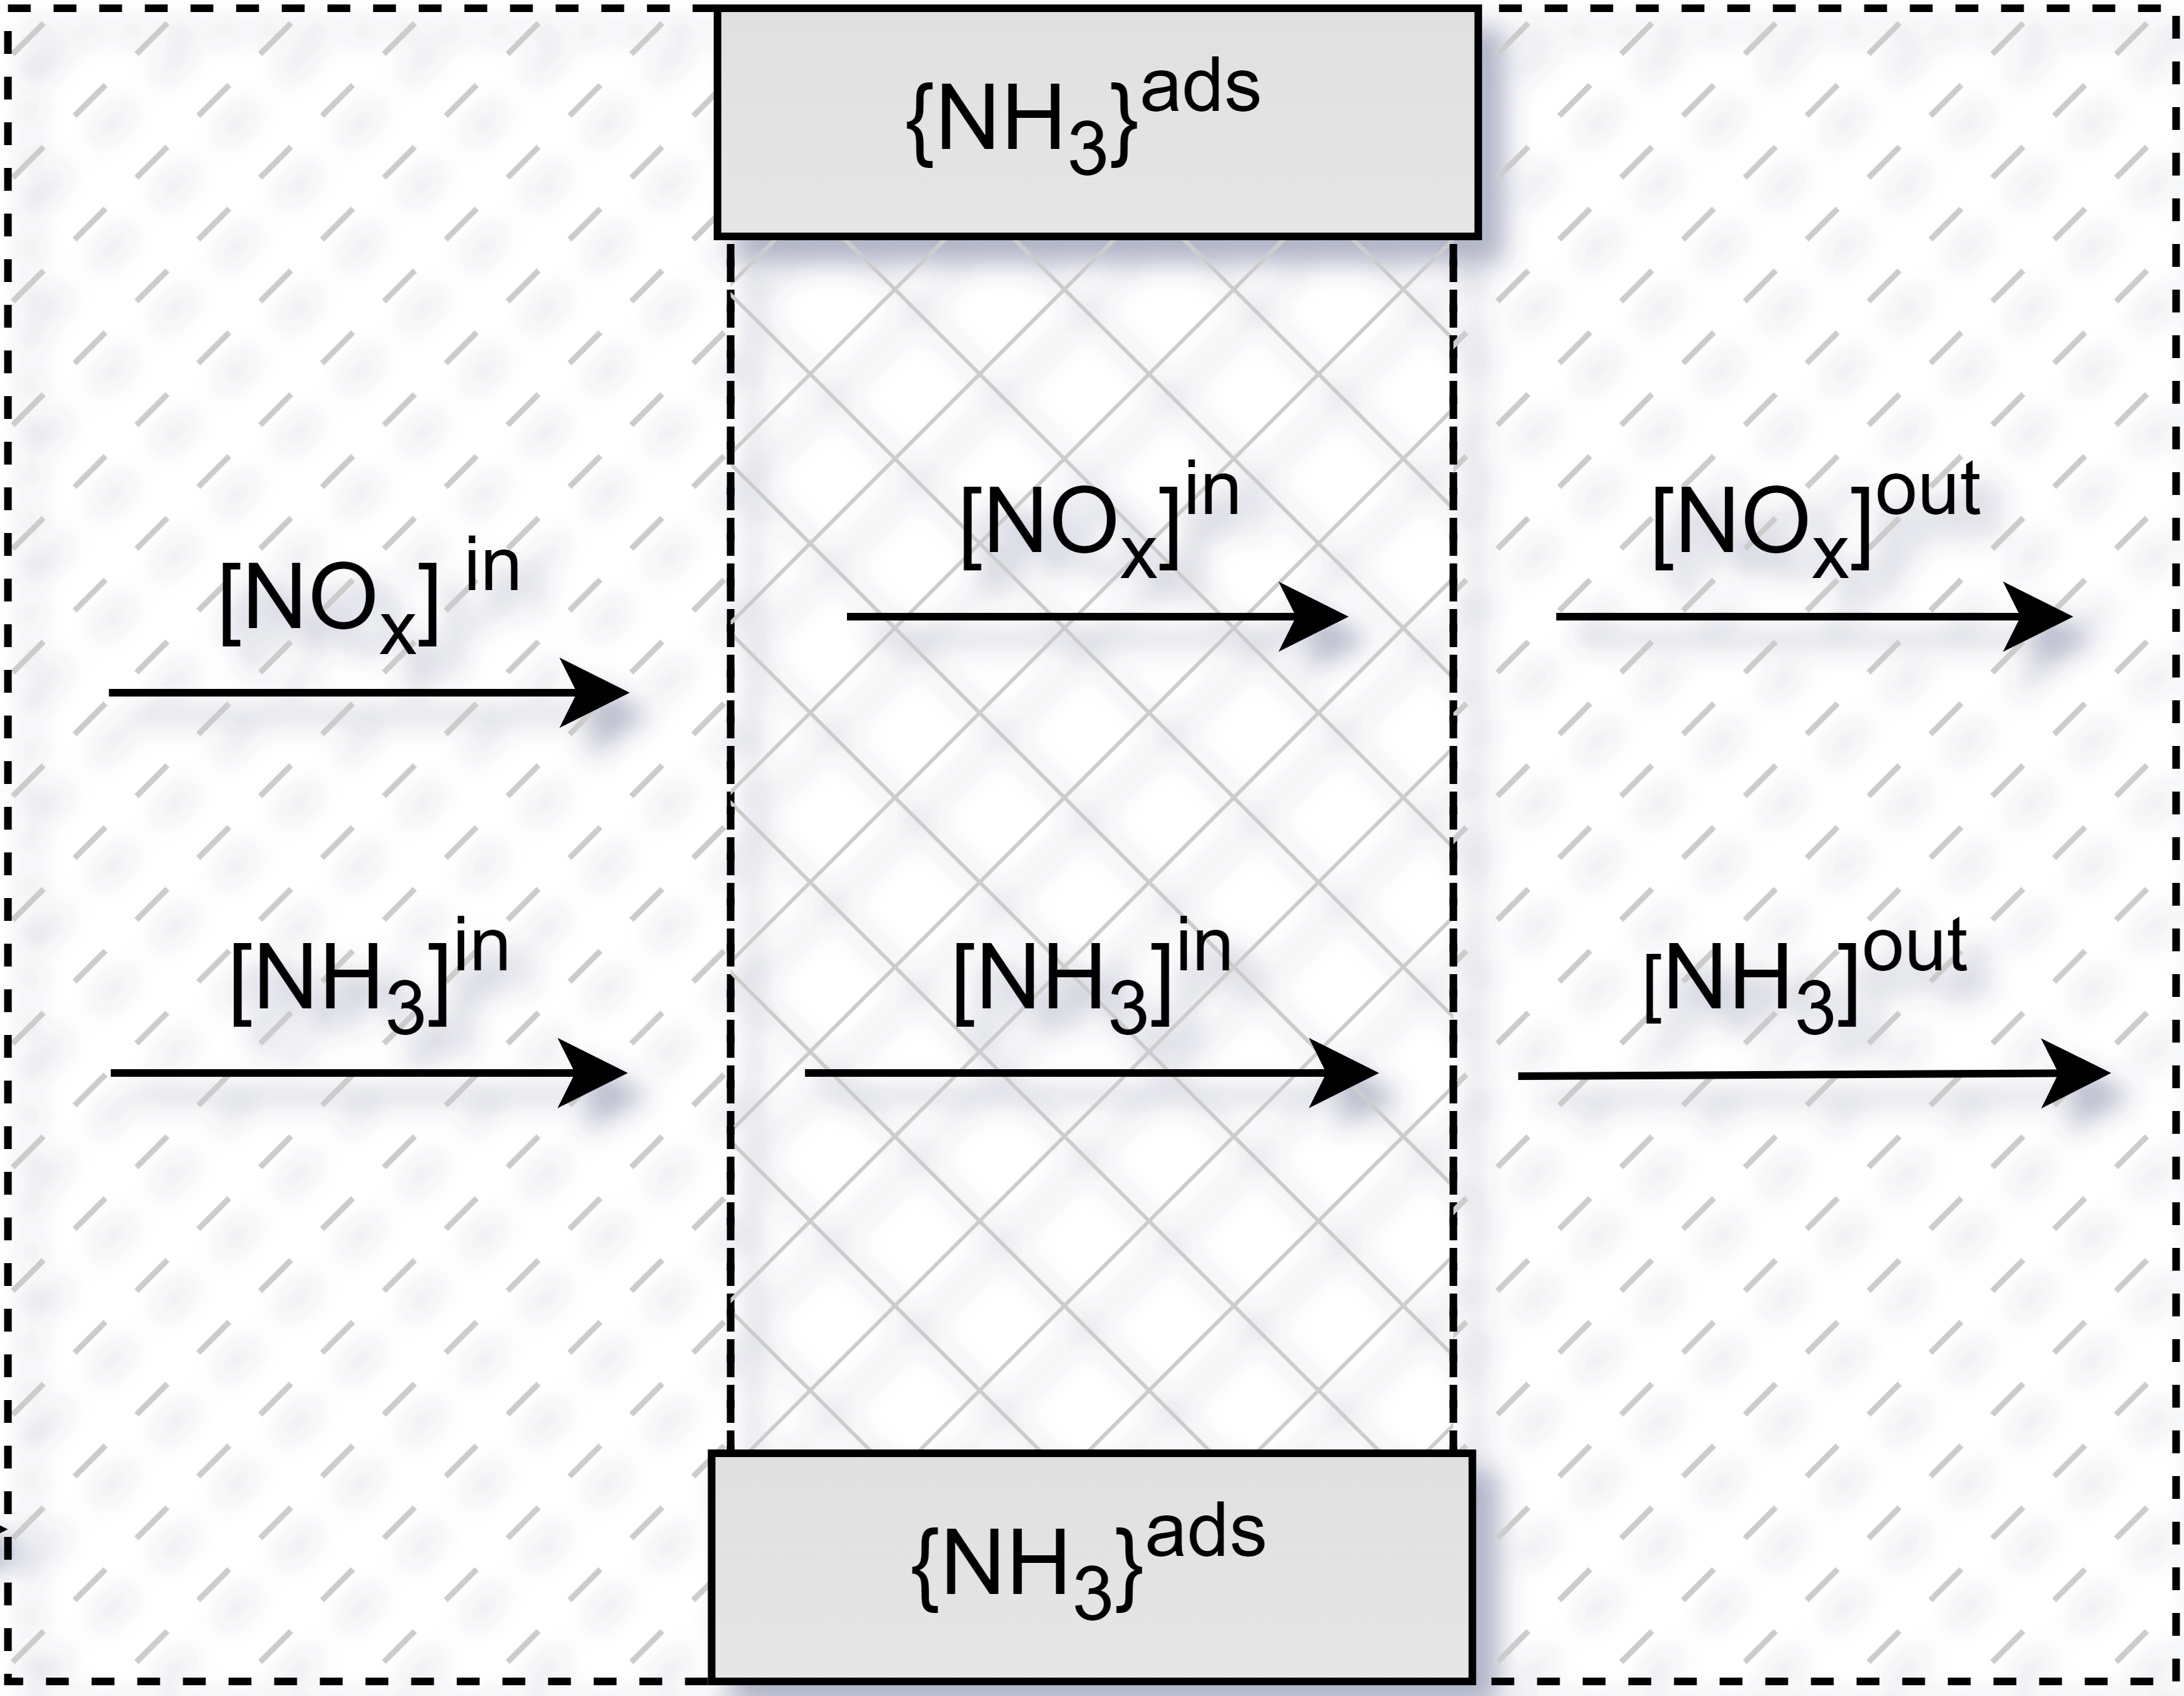
\includegraphics[width=0.35\textwidth]{figs/2_mdl/plug_flow_discrete.png}
    \caption{Approximating the plug flow reaction}
    \label{fig:plug-flow}
\end{figure}
%===
%% 1. The NO_x reduction dynamics are different when the Catalyst is saturted as it is independent of the urea-dosing.
%====
Considering the reaction chamber as a control volume (Figure-\ref{fig:plug-flow}), the dynamic model is developed based
on the molar conservation of species at the inlet and outlet separated by a residence-time interval. By assuming a
zero-order hold on the inlet species over the sampling time, the equations relating inlet and outlet concentrations at
the residence-time scale are extended to the sampling-time scale.
%====
% ======================================================================================================================
% \subsection{$NO_x$ PROCESS DYNAMICS}
Let, $\lrf{\bullet}$ be the number of moles and $\lrb{\bullet}$ be the concentration of a given species $\bullet$. We have the molar conservation of $NO_x$ across the control volume $(V_{scr})$ within one residence time $(\tau)$:
%====
\begin{multline}
        \mol{NO_x}^{out} (t + (i+1) \tau) =
                \mol{NO_x}^{in} (t + i \tau) \\
                + V_{scr} \int_0^{\tau} \frac{d}{dt} \con{NO_x}^{scr}dt
        \label{eqn::nox_bal}
\end{multline}
%===
The number of moles entering at the inlet and leaving at the outlet can be written as a function of the concentration, residence time and volume flow rate $(F_{vol})$:
%===
\begin{align}
    \mol{NO_x}^{in/out} = \con{NO_x}^{in/out} \tau F_{vol} = \con{NO_x}^{in/out} V_{scr}
\end{align}
%===
Using Eiley-Rideal mechanism for Standard SCR reaction $\lrf{2}$:
\begin{align}
    \frac{d}{dt} \con{NO_x}^{scr}dt = -k_{scr} \con{NH_3}^{ads} \con{NO_x}^{in}
\end{align}
%===
Rewriting (\ref{eqn::nox_bal}) in terms of concentrations and integrating to residence time:
\begin{multline}
        \con{NO_x}^{out} (t + (i+1) \tau) =
                \con{NO_x}^{in} (t + i \tau) \\
                -\tau k_{scr} \con{NH_3}^{ads} \con{NO_x}^{in}
        \label{eqn::nox_bal_con}
\end{multline}
%====
Summing the equations from (\ref{eqn::nox_bal_con}) for  $i = 0$ to $n-1$, where $n$ is the total number of residence times within one sampling period $(n= t_s/\tau)$ and using the zero-order hold assumptions at the inlet (\ref{eqn::zero_in}) and outlet (\ref{eqn::zero_out}) concentrations, we get equation (\ref{eqn::nox_avg}).
\begin{align}
    \con{NO_x}^{in} (t + i \tau) &= \con{NO_x}^{in}(t) \quad \forall i \in [0, n-1]  \label{eqn::zero_in}\\
    \con{NO_x}^{out} (t + (i+1) \tau) &= \con{NO_x}^{out}(t + t_s) \quad \forall i \in [0, n-1] \label{eqn::zero_out}
\end{align}
\begin{multline}
        \underbrace{\con{NO_x}^{out}}_{x_1(k+1)}(t+t_s) =
                \underbrace{\con{NO_x}^{in}}_{u_1(k)}(t) \\
                - \tau(t) k_{scr}(t) \con{NO_x}^{in}(t) \underbrace{\lrf{\frac{1}{n} \sum_{i = 0}^{n-1} \con{NH_3}^{ads}(t + i \tau)}}_{\sigma(k)}
        \label{eqn::nox_avg}
\end{multline}
%
% ======================================================================================================================
%
The quantity $\sigma(k)$ is the average concentration of ammonia adsorbed on the catalysts surface across the $n$ residence times between $k$ and $k+1$ samples. $\sigma(k)$ is bounded by the total concentration of voids on the surface of the catalyst, $\Gamma$, which decrease with increase in temperature.
\begin{align}
    0 \leq \sigma(k) \leq \Gamma \qquad \forall k
\end{align}
%===
The unbounded dynamics of $\sigma$, $\sigma^{ub}(k)$ is a nonlinear function dependent on concentration of adsorbed ammonia, urea dosing $\lr{u_{inj}}$, and the inlet $NO_x$ concentration from the previous time step.
\begin{align}
    \sigma^{ub}(k) &= g_{\sigma} \lr{ \sigma(k-1), u_{inj}(k-1), \con{NO_x}^{in}(k-1) }
\end{align}
The actual expression, which is beyond the scope of this work, can be derived using the similar approach used for
deriving $NO_x$ process dynamics (\ref{eqn::nox_avg}). $\sigma(k)$ can be described using the following pairwise
function:
\begin{align}
    \sigma(k) &=
    \begin{cases}
        \sigma^{ub}(k) & \text{if } \quad 0 \leq \sigma^{ub}(k) \leq \Gamma \\
        \Gamma         & \text{if } \quad \sigma^{ub}(k) > \Gamma \qquad \text{[Satuaration]}\\
        0              & \text{if } \quad \sigma^{ub}(k) < 0 \qquad \text{[Empty]}
    \end{cases}
\end{align}
%===
Thus, for $NO_x$ process dynamics under catalyst saturation, $\sigma(k) = \Gamma$. From (\ref{eqn::nox_avg})
\begin{align}
    x_{1_{sat}}(k+1) &= u_1(k) - \underbrace{\tau(k) k_{scr}(k) u_1(k) \Gamma}_{\bm{\text{$NO_x$ reduction in} \\\text{sampling period $\lr{\eta(k)}$}}}
        \label{eqn::nox_mdl}
\end{align}
%===
The above equation~(\ref{eqn::nox_mdl}) shows that the tailpipe $NO_x$ concentration becomes independent of urea dosing under catalyst saturation. Defining $\eta(k)$ as change in $NO_x$ concentration reduction during the time between $k-1$ and $k$, i.e.,
\begin{align}
    \eta_{sat}(k) &= u_1(k-1) - x_{1_{sat}} (k)
    \label{eqn::eta}
\end{align}
%===
The residence time can be parameterized as a function of mass flow rate $\lr{F}$ assuming that the effect of the density variation on residence time is insignificant.
\begin{align}
    \tau(k) &= \frac{\rho V_{scr}}{F} = \frac{\tau_0}{F}
    \label{eqn::res_time}
\end{align}
%===
The temperature dependence of the rate constant, $k_{scr}$, can be approximated by linearizing Arrhenius equation as:
\begin{align}
    k_{scr}(T) = A_{scr} e^{\lr{-\frac{E_{scr}}{RT}}} \approx k_1 T + k_0 \qquad k_1, k_0 > 0
    \label{eqn::rate_const}
\end{align}
%===
The temperature model for concentration of viable voids $\Gamma$ on the catalyst \cite{nova2014urea},\cite{ciardelli2004scr}, \cite{joo2008study} is approximated as a linear function that decreases with increase in temperature.
:w
\begin{align}
    \Gamma(T) &= S_1 e^{-S_2 T} \approx -\gamma_1 T + \gamma_0 \qquad \gamma_1, \gamma_0 > 0
    \label{eqn::gamma}
\end{align}
%===
Incorporating equations (\ref{eqn::eta}), (\ref{eqn::res_time}) and (\ref{eqn::gamma}) into the $NO_x$ process dynamic model (\ref{eqn::nox_mdl}) and writing in regression form, we get
\begin{align}
    \eta_{sat}(k+1) &= \pmb \phi_{sat}^T(k) \pmb \theta_{sat}
    \label{eqn::regression} \\
    %===
    \pmb \phi_{sat} (k) &= \frac{u_1(k)}{F(k)} \times \bm{T^2 \\ T \\ 1}
    \label{eqn::phi_def}\\
    %===
    \pmb \theta_{sat} &= \tau_0 \times \bm{-k_1 \gamma_1 \\ k_1 \gamma_0 - k_0 \gamma_1 \\ k_0 \gamma_0}
                       = \bm{\theta_1 \\ \theta_2 \\ \theta_2}
    \label{eqn::theta_def}
\end{align}
%===
Based on the parameter definitions (\ref{eqn::theta_def}), the signs of two of the parameters is deterministic.
\begin{align}
    \theta_1 \leq 0, \qquad
    \theta_3 \geq 0
\end{align}

%===
%% 2. The I/O dynamics for NO_x reduction under Catalyst Saturation forms an upper bound to the actual NO_x reduction dynamics which switch between Saturation and de-saturation.
%===
It can be observed that, in a given time step maximum $NO_x$ reduction happens when the catalyst is saturated. Thus,
under the same temperature, flow rate and inlet $NO_x$ concentration, the response of the saturated model
(\ref{eqn::eta}) forms a tight upper bound to the response of the actual system, that switched between saturation and
desaturation based on urea dosing.
%===
\begin{align}
        \eta_{sat}(k) \geq \eta(k) \qquad \forall k
        \label{eqn::eta_bound}
\end{align}
%===
This relationship can is used for model parameter estimation.

%===

\section{Model Parameter Estimation Algorithm and Validation}
The parameters of the $NO_x$ process dynamics under catalyst saturation (\ref{eqn::eta}), are estimated using the bounding constraint (\ref{eqn::eta_bound}) on the experimental data. The parameters are the solution of the following optimization problem:
\begin{align}
\text{minimize} &\qquad \sum_{k=1}^{N} \lr{ \eta_{sat}(k) - \eta(k)} ^2 \\
\text{subject to} &\qquad \eta_{sat}(k) \geq \eta(k) \quad \forall \, k \in \lrf{1,2,\hdots, N} \notag
\end{align}
%===
The above constrained least-squares problem can also be posed as an equivalent linear programming problem as $\eta_{sat}, \eta \geq 0$ always. The solution provides the system's parameter estimates under ideal conditions, i.
e., in the absence of model structure uncertainties and measurement noise.

\section{Model Parameter Estimation under $NO_x$ Sensor Cross-sensitivity}

\section{Application 1: Catalyst Mode Detection}

\section{Application 2: Catalyst Aging Detection}

\section{Conclusion}


%=======================================================================================================================
\section*{Acknowledgment}
Authors acknowledge the support and feedback from David Schmidt, Larry Bruner, Adam Kidd and Tom Nelson of Cummins, Inc.
%=======================================================================================================================
\section*{Funding Data}
Authors acknowledge the funding and test-cell, truck and simulation data of Diesel Engine Aftertreatment Systems from Cummins, Inc.
%=======================================================================================================================
\appendix   %%% starting appendices
\section{APPENDIX-A: List of Symbols}
%\EntryHeading{Greek Letters}

\begin{nomenclature}
    \entry{$\lrf{\bullet}$}{Number of moles of $\bullet$. $(moles)$}
    \entry{$\lrb{\bullet}$}{Concentration of $\bullet$. $(mol/m^3)$}
    \entry{$\Gamma $}{Surface concentration of the total storage capacity for the catalyst $(mol/m^2)$}
    \entry{$E_{scr}$}{Activation Energy of SCR reaction}
    \entry{$A_{scr}$}{Pre-exponential factor of SCR reaction}
    \entry{$R$}{Universal gas constant}
    \entry{$T$}{Temperature}
    \entry{$k_1, k_2$}{Coefficients of linear temperature model for $k_{scr}$, $k_1, k_2 \geq 0$.}
    \entry{$S_1, S_2$}{Coefficients of the temperature model for $\Gamma$, $S_1, S_2 \geq 0$}
    \entry{$\gamma_1, \gamma_2$}{Coefficients of linear temperature model for $\Gamma$, $\gamma_1, \gamma_2 \geq 0$}
    \entry{$V_{scr}$}{Volume of the catalyst chamber}
    \entry{$F$}{Mass flow rate of the exhaust gases $(g/s)$}
    \entry{$\rho$}{Density of the exhaust gases}
    \entry{$\sigma(k)$}{Average surface concentration of adsorbed ammonia in the sample [k] to [k+1]}
\end{nomenclature}


\section{APPENDIX-B: Relevant Mathematical Results}
\begin{lemma}
        \label{lemma::T_suff}
\end{lemma}


%=======================================================================================================================
\bibliographystyle{asmejour}
\bibliography{refs}
\end{document}
